%!TEX root = SSCR_project_main.tex
\chapter{Design}
An initial UML class diagram was made, and later refined during the implementation. 
In Figure \ref{fig:ClassDiagram} the final class diagram is shown.

\begin{figure}[H]
\centering
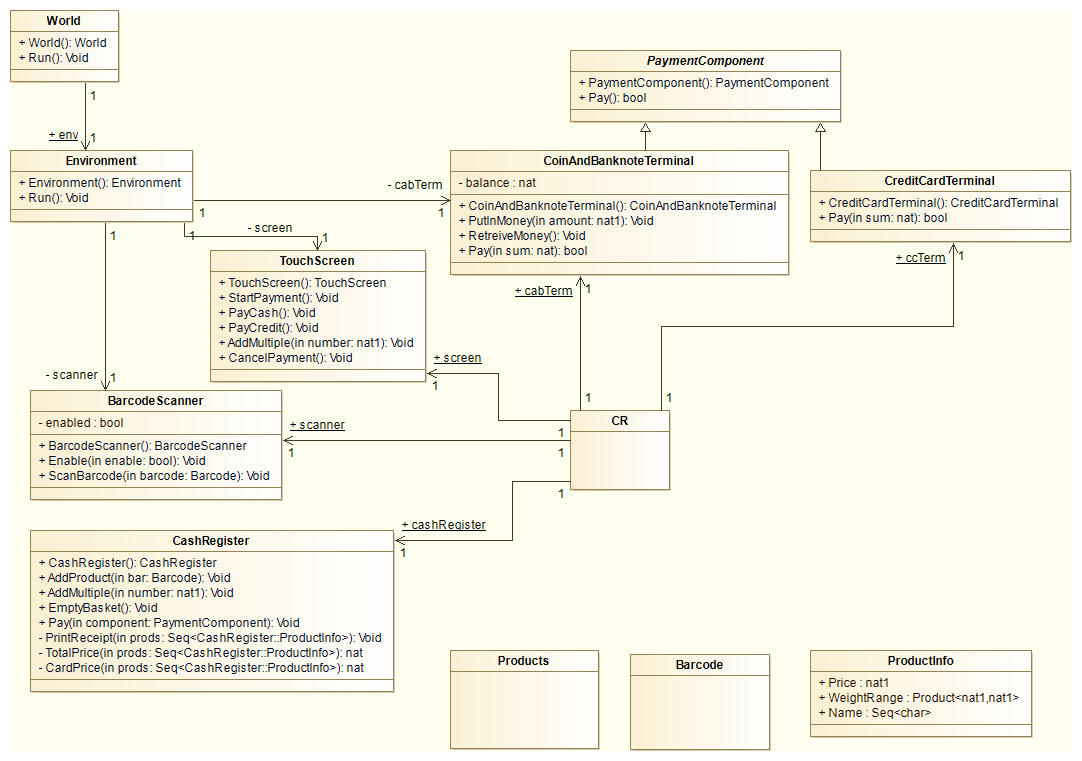
\includegraphics[width=\linewidth]{ClassDiagram}
\caption{Final class diagram.}
\label{fig:ClassDiagram}
\end{figure}

The CR class is the 'system' class, which contains static references to all of the systems objects. 
The World and Environment classes are used to create stimuli to the system.

The CashRegister class contains most of the functionality. It is also this class that contains a database of all products and corresponding barcodes. 
It also contains a list of items in the 'shopping cart' and the accumulated price for the scanned products.